\def\mytitle{TRIANGLES}
\documentclass[10pt,a4paper]{article}
\usepackage{graphicx}
\graphicspath{{./images/}}
\usepackage[colorlinks,linkcolor={black},citecolor={blue!80!black},urlcolor={blue!80!black}]{hyperref}
\usepackage[parfill]{parskip}
\usepackage{lmodern}
\usepackage{tikz}
\usepackage{physics}
\usepackage{tabularx}
\usepackage{enumitem}
\usetikzlibrary{calc}
\usepackage{amsmath}
\usepackage{amssymb}
\renewcommand*\familydefault{\sfdefault}
\usepackage{watermark}
\usepackage{lipsum}
\usepackage{xcolor}
\usepackage{listings}
\usepackage{float}
\usepackage{titlesec}
\providecommand{\mtx}[1]{\mathbf{#1}}
\titlespacing{\subsection}{1pt}{\parskip}{3pt}
\titlespacing{\subsubsection}{0pt}{\parskip}{-\parskip}
\titlespacing{\paragraph}{0pt}{\parskip}{\parskip}


\newcommand{\myvec}[1]{\ensuremath{\begin{pmatrix}#1\end{pmatrix}}}
\let\vec\mathbf
\lstset{
frame=single, 
breaklines=true,
columns=fullflexible
}
\title{\mytitle}
\begin{document}
	\maketitle
	\tableofcontents
	
\section{Problem}	
In the given figure,$AC =AE$,$AB=AD$ and $\angle BAD=\angle EAC$.Show that $BC=DE$.
\begin{figure}[!h]
	\begin{center}
		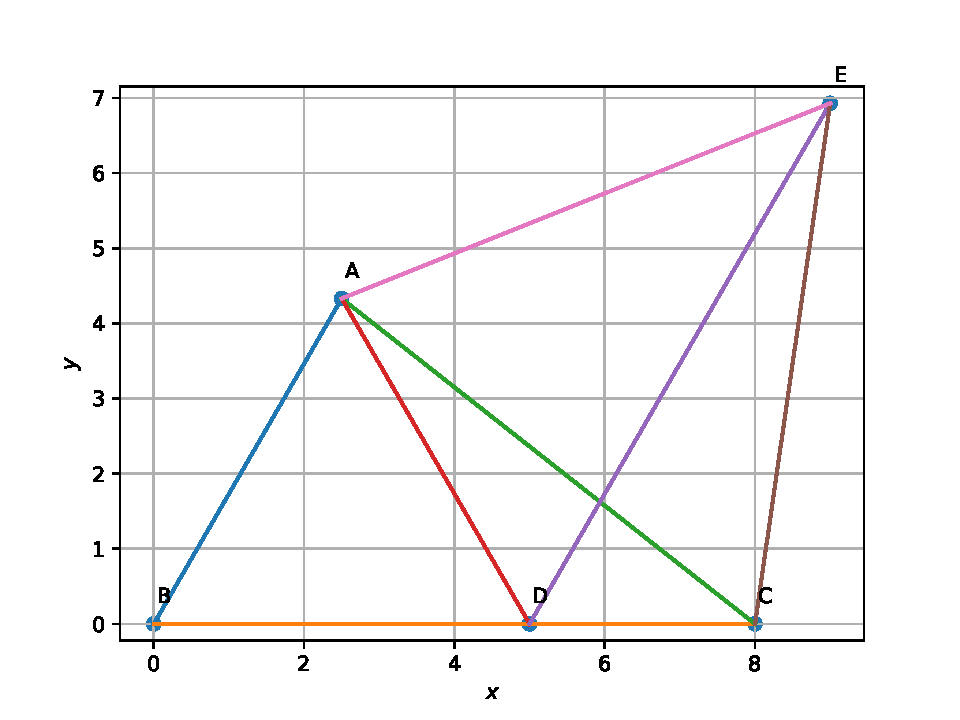
\includegraphics[width=\columnwidth]{./fig/fig.pdf}
	\end{center}
\caption{}
\label{figure}
\end{figure}


\section{Construction}

\begin{center}

The input parameters for this construction are

\begin{tabular}{|c|c|}
	\hline
	\textbf{Symbol}&\textbf{Value}\\
	\hline
	r&3\\
	\hline
    b&4\\
    \hline
	b1&3\\
	\hline
	$\theta1$&$\frac{pi}{3}$\\
	\hline
	$\theta2$&$\frac{pi}{4}$\\
	\hline
	
\end{tabular}
\end{center}

\begin{align*}
\vec{A}=\begin{pmatrix} r\cos\theta\\ r\sin\theta\ \end{pmatrix} \\
\vec{B}=\begin{pmatrix} 0\\ 0\ \end{pmatrix} \\
\vec{C}=\begin{pmatrix} 4\\ 0\ \end{pmatrix} \\
\vec{D}=\begin{pmatrix} 3\\ 0\ \end{pmatrix} \\
\vec{E}=\begin{pmatrix} 4.1\\ 4\ \end{pmatrix} \\
\end{align*}

\section{Solution}
 We know that two triangles are  said to be congruent if the sides and angles of one
triangle are equal to the corresponding sides and angles of the other triangle.In congruent triangles corresponding parts are equal.

\paragraph{Given}
\begin{align}
\vec{A}-\vec{C} &=\vec{A}-\vec{E} \\
\vec{A}-\vec{B} &=\vec{A}-\vec{D}\\
\angle BAD &=\angle EAC
\end{align}
	

\textbf{Proof}\\
Given that
\begin{align*}
\angle BAD &=\angle EAC\\
\angle BAD+\angle DAC &=\angle EAC+\angle DAC\\
\angle BAC &=\angle DAE\\
\end{align*}


In $\triangle ABC $ and in $\triangle ADE$

\begin{align}
\vec{A}-\vec{B}&=\vec{A}-\vec{D}
\label{fig:9/8/1/9/pgm}\\
\angle BAC &=\angle DAE\\
\implies cos \angle BAC &=cos \angle DAE\\
\begin{split}
\implies \frac{(\vec{A}-\vec{B})^T(\vec{A}-\vec{C})}{\norm{\vec{A}-\vec{B}}\norm{\vec{A}-\vec{C}}} &=
\frac{(\vec{A}-\vec{D})^T(\vec{A}-\vec{E})}{\norm{\vec{A}-\vec{D}}\norm{\vec{A}-\vec{E}}}
\end{split}
\label{fig:9/8/1/9/newpgm}\\
\vec{A}-\vec{C}&=\vec{A}-\vec{E}
\label{fig:9/8/1/9/newpgmsol}
\end{align}

	
\begin{enumerate}
    \item From 
		\eqref{fig:9/8/1/9/pgm}, 
		\eqref{fig:9/8/1/9/newpgm}
		and 
		\eqref{fig:9/8/1/9/newpgmsol}
		
		taking the norms of the respective sides, 
    \begin{align}
        \triangle ABC \cong \triangle ADE
    \end{align}
    
\item From  
		\eqref{fig:9/8/1/9/pgm}, 
		\eqref{fig:9/8/1/9/newpgm}
		and 
		\eqref{fig:9/8/1/9/newpgmsol}
 taking the norms of the respecttive sides
 \begin{align}
BC=DE
 \end{align}    
\end{enumerate}
\end{document}
\fi
